%----------------------------------------------------------------------------
%Type of document
\documentclass{beamer}

%----------------------------------------------------------------------------
%Packages
\usepackage{amsmath}
\usepackage{hyperref}
\usepackage{subfigure}
\usepackage{graphicx}
\usepackage{centernot}
\usepackage{appendixnumberbeamer}

%----------------------------------------------------------------------------
%Local adjustments of settings and definitions
\setcounter{MaxMatrixCols}{10}
\setbeamertemplate{caption}[numbered]
\definecolor{links}{HTML}{2A1B81}
\hypersetup{colorlinks,linkcolor=,urlcolor=links}

%----------------------------------------------------------------------------
%Beamer theme (Madrid and Frankfurt are good options)
\usetheme{Madrid}

%----------------------------------------------------------------------------
%Start document
\begin{document}

%----------------------------------------------------------------------------
%Front matter
\title[Monetary Policy]{Monetary Policy - Conventional and Unconventional}
\author[Bidder]{Rhys Bidder}
\institute[FRBSF]{Federal Reserve Bank of San Francisco}
\date{Michaelmas Term 2019}
\maketitle

%----------------------------------------------------------------------------
%Main body

\begin{frame}{Disclaimer}

The views expressed in this presentation, and all errors and omissions, should be regarded as those solely of the authors, and are not necessarily those of the Federal Reserve Bank of San Francisco, the Federal Reserve Board of Governors or the Federal Reserve System.

\end{frame}

%-------------------------------------------------------
\section{Monetary Policy in the New Keynesian Model}
%-------------------------------------------------------

\begin{frame}

\begin{center}
{\LARGE Monetary Policy in the NK Model}
\end{center}

\end{frame}

%-------------------------------------------------------

%-------------------------------------------------------

\begin{frame}{Monetary Policy in the New Keynesian Model}

\begin{itemize}
\item	We have shown that monetary policy can have real effects in the New Keynesian model
\item	We also note that the New Keynesian model features distortions that lead to inefficiencies
\item	Ability to affect an economy featuring inefficiencies $\Rightarrow$ possible role for policy interventions
\item	Central banks are heavy users (and developers of) New Keynesian models
\item	Structural models allow policymakers to understand and plan the effects of policy
\end{itemize}

\end{frame}

%-------------------------------------------------------

%-------------------------------------------------------
	
\begin{frame}{Steady state (in)efficiency in the NK model}

Recall from the previous lecture:
\begin{itemize}
\item	Steady state value of $y^{n}_{t}$ (and $y_{t}$) was lower than in Classical model
\item	Related to the pricing power of monopolistically competitive firms
\item	Markup: $\mu \equiv \log{(\mathcal{M})} \equiv \log{(\frac{\varepsilon}{\varepsilon-1})}$
\end{itemize}

\vspace{2mm}
Natural rate of output in NK model
\begin{eqnarray*}
y^{n}_{t} 	&=& 		\psi_{yn} + \psi_{yn,a} a_{t} \\
\psi_{yn}	&\equiv& 	-\frac{(1-\alpha)(\textcolor{red}{\mu}-\log{(1-\alpha)})}{\sigma(1-\alpha)+\varphi+\alpha}
\end{eqnarray*}

Output in Classical model
\begin{eqnarray*}
y^{c}_{t} 		&=& 		\psi_{yc} + \psi_{yc,a} a_{t} \\
\psi_{yc} 		&\equiv& 	\frac{(1-\alpha)\log{(1-\alpha)}}{\sigma(1-\alpha)+\varphi+\alpha} \\
\end{eqnarray*}

\end{frame}

%-------------------------------------------------------

%-------------------------------------------------------
	
\begin{frame}[label=efficiency]{Inefficiency in the NK model}

Monetary policy is not the `right' tool to correct industrial structure inefficiencies
\begin{itemize}
\item	Can't fix monopolistic competition
\item	Need to rely on supply side (e.g. tax/subsidy policies)
\item	In an earlier homework we showed that if producers are subsidized appropriately, we can recover the efficient level of output \hyperlink{efficiency_escape}{\beamergotobutton{More detail}}
\item	We will assume such a policy holds, so the \textbf{`steady state'} value of $y_{t}$ and both the steady state \textit{and current values} of $y^{n}_{t}$ are efficient
	\begin{itemize}
	\item	Flexible prices in the `natural rate' world $\Rightarrow$ if we fix competitive distortions, there's nothing left to cause inefficiency, in or out of steady state
	\end{itemize}
\end{itemize}

\vspace{2mm}
But that's not the end of the story\ldots

\end{frame}

%-------------------------------------------------------

%-------------------------------------------------------
	
\begin{frame}{Inefficiency in the NK Model}

Additional conditions that must be satisfied by an efficient allocation are\ldots

\vspace{2mm}
\begin{itemize}
\item	All goods (indexed by $i$) should be consumed (and thus produced) in the same quantities
\[
C_{t}(i) = C_{t}\text{  } \forall i \in [0,1]
\]

\item	All firms (each identified with a good, $i$) should employ the same amount of labor
\[
N_{t}(i) = N_{t}\text{  } \forall i \in [0,1]
\]

\end{itemize}

\end{frame}

%-------------------------------------------------------

%-------------------------------------------------------
	
\begin{frame}{An efficient benchmark}

Under the flex-price equilibrium or the zero inflation steady state of the sticky price model
\vspace{2mm}
\begin{itemize}
\item	All firms are producing the same amounts
	\begin{itemize}
	\item	Why? They face the same technology and prices
	\end{itemize}
\item	Each (identical) household consumes the same amount of each good
	\begin{itemize}
	\item	Why? All goods have the same price and enter symmetrically in the concave utility function
	\end{itemize}
\end{itemize}

\vspace{3mm}
But price stickiness prevents this from holding \textit{outside the steady state} from period to period

\end{frame}

%-------------------------------------------------------

%-------------------------------------------------------
	
\begin{frame}{An efficient benchmark}

Even if the \emph{steady state} of the NK model is efficient under the subsidy this does not mean it is efficient in any given period

\vspace{2mm}
\begin{itemize}
\item	Due to price stickiness, the average markup will vary over time
	\begin{itemize}
	\item	Average marginal cost will vary with average scale of production
	\item	Prices do not adjust fully to reflect this
	\item	Even if a constant subsidy is adjust for steady state markups, it can't correct for \textit{variations} in markups
	\item	Remember markups ($P \neq MC$) are associated with inefficiency
	\end{itemize}
	\vspace{2mm}
\item	\textbf{Due to price stickiness there will be dispersion in prices}
	\begin{itemize}
	\item	Leads to dispersion in consumption and employment across firms/goods
	\item	Violates optimality conditions for consumption and resource allocation
	\item	But this \textbf{\textit{is}} something monetary policy can rectify, in theory
	\end{itemize}
\end{itemize}

\end{frame}

%-------------------------------------------------------

%-------------------------------------------------------
	
\begin{frame}{Optimal Allocation}

Suppose we start from a steady state situation
\begin{itemize}
\item	All firms were setting the same price in the previous period
\item	Price was at desired markup over (subsidy adjusted) marginal cost
\item	All firms operate on the same scale
\item	Goods are consumed in the same quantity
\item	Output is at its natural level
\end{itemize}

\end{frame}

%-------------------------------------------------------

%-------------------------------------------------------
	
\begin{frame}{Optimal Allocation}

If shocks hit the economy, how should policy respond?
\begin{itemize}
\item	The aim is to preserve $y_{t} = y^{n}_{t}$ (or $\tilde{y}_{t}=0$) since $y_{t}^{n}$ is efficient
\item	Since this must be part of an equilibrium, the NKPC must hold
\item	Iterating the NKPC forwards $\Rightarrow$ if $ \tilde{y}_{t}=0$ $\forall t$ then $\pi_{t}=0$ $\forall t$
\end{itemize}
\begin{eqnarray*}
\pi_{t} 	&=& \beta E_{t}[\pi_{t+1}] + \kappa \tilde{y}_{t}	\\
		&=& \beta E_{t}[ \beta E_{t+1}[\pi_{t+2}] + \kappa \tilde{y}_{t+1}] + \kappa \tilde{y}_{t} \\
		&\ldots&	\\
		&=& \kappa \sum\limits_{j=0}^{\infty} \beta^{j} E_{t}[\tilde{y}_{t+j}]
\end{eqnarray*}

\end{frame}

%-------------------------------------------------------

%-------------------------------------------------------
	
\begin{frame}{Optimal Allocation}

From an alternative perspective\ldots
\begin{itemize}
\item	Assume $\pi_{t}=0$ $\forall t$ and all firms are initially at their desired markup
\item	If policy is such that marginal cost is stabilized, then the existing price will continue to be optimal
	\begin{itemize}
	\item	Since the markup is already at desired level and the marginal cost to which the markup is applied is unchanged
	\end{itemize}
\item	No firm (even the $1-\theta$ who \emph{can} reset) will want to change their price
	\begin{itemize}
	\item	Thus inflation will be zero
	\item	Price stickiness irrelevant (like being in flex price)
	\end{itemize}
\item	Output is equal to natural $\Rightarrow$ constant real marginal cost
	\begin{itemize}
	\item	Thus, under zero inflation, we have constant nominal marginal cost
	\item	Justifies firms not changing prices
	\end{itemize}
\end{itemize}

\vspace{2mm}
If policy achieves price stability then it also coincidentally achieves $y_{t}=y^{n}_{t}$
\begin{itemize}
\item	\textcolor{red}{`Divine coincidence'}
\item	No trade-off between price stability and goals for $y_{t}$
\end{itemize}

\end{frame}

%-------------------------------------------------------

%-------------------------------------------------------
	
\begin{frame}{Optimal Allocation}

Note that efficiency does not imply constant activity
\begin{itemize}
\item	$MC_{t}$ is stabilized such that the desired markup $\Rightarrow$ constant $P_{t}$
\item	But \emph{output} can still vary in an efficient allocation
	\begin{itemize}
	\item	$\tilde{y}_{t}=0 \Rightarrow y_{t} = y^{n}_{t}$
	\item	$y^{n}_{t}$ depends on $a_{t}$
	\end{itemize}
\item	This reflects one of the main insights of the RBC literature (business cycles $\centernot\implies$ market failure)
\end{itemize}

%Same markup and same p(t) means mc must be constant. If mpn(t) changes with yn(t) then w must be changing. If mpn(t) is constant then wage need not change in equilibrium.

\end{frame}

%-------------------------------------------------------

%-------------------------------------------------------
	
\begin{frame}{Optimal Allocation}

Nice quote from Gal\'i p. 104

\begin{quotation}
The intuition behind the desirability of zero inflation in the case of an efficient natural allocation can be conveyed as follows: if price stability is attained, then it must be the case that no firm is adjusting its price even when having the option to do so, from which it follows that the constraints on price setting are not binding and, hence, that the equilibrium allocation corresponds to that of an economy with flexible prices (which is, under the assumptions made here, efficient).
\end{quotation}

\end{frame}

%-------------------------------------------------------

%-------------------------------------------------------
	
\begin{frame}{Optimal Policy}

What interest rate policy is consistent with the optimal allocation as an \emph{equilbrium} outcome?
\begin{itemize}
\item	$y_{t}=y^{n}_{t}$ combined with the DIS curve implies $r_{t} = r^{n}_{t}$
\item	Zero inflation $\forall t$ implies $i_{t} =  r_{t}$ (by the Fisher equation)
\end{itemize}

\vspace{2mm}
Thus under optimal policy, in equilibrium,
\begin{equation}
i_{t} = r^{n}_{t}	\label{eqn:ir_rnt}
\end{equation}

\vspace{2mm}
But is this an adequate \emph{rule} for how the interest rate should be set in all contingencies?

\end{frame}

%-------------------------------------------------------

%-------------------------------------------------------
	
\begin{frame}{Optimal Policy}

$i_{t}=r^{n}_{t}$ holds in our desired equilibrium with $\tilde{y}_{t}=\pi_{t}=0$
\begin{itemize}
\item	But it \emph{also} can hold in other less desirable equilibria
\item	In these equilibria we do not have $\tilde{y}_{t}=\pi_{t}=0$
\item	Thus we lose the desired efficiency properties
	\begin{itemize}
	\item	We can have $i_{t}=r^{n}_{t}$ but if $\pi_{t}\neq0$ $\forall t$ then $r_{t}$ will deviate from $r^{n}_{t}$
	\item	Then we cannot guarantee that $y_{t}=y^{n}_{t}$ $\forall t$
	\end{itemize}
\end{itemize}

\vspace{2mm}
Equation (\ref{eqn:ir_rnt}) derived `assuming' optimal allocation ($\tilde{y}_{t}=\pi_{t}=0$ $\forall t$)
\begin{itemize}
\item	Doesn't allow for possibility of deviations from the optimal allocation
\item	This `opens the door' to alternative allocations
\item	Needs to be augmented with response to `off equilibrium' outcomes
\end{itemize}

\end{frame}

%-------------------------------------------------------

%-------------------------------------------------------
	
\begin{frame}{Optimal Policy}

Consider instead two alternative rules
\vspace{2mm}
\begin{itemize}
\item	A rule that responds to realized inflation and activity
\[
i_{t} = r^{n}_{t} + \phi_{\pi} \pi_{t} + \phi_{y} \tilde{y}_{t}	
\]
\item	A rule that responds to forecasts/expectations of inflation and activity
\[
i_{t} = r^{n}_{t} + \phi_{\pi} E_{t}[ \pi_{t+1} ] + \phi_{y} E_{t}[ \tilde{y}_{t} ]
\]
\end{itemize}

Let us simplify these rules further
\begin{eqnarray*}
i_{t} &=& r^{n}_{t} + \phi_{\pi} \pi_{t} 				\label{eqn:taylor_1} \\
i_{t} &=& r^{n}_{t} + \phi_{\pi} E_{t}[ \pi_{t+1} ]		\label{eqn:taylor_2}
\end{eqnarray*}

\end{frame}

%-------------------------------------------------------

%-------------------------------------------------------
	
\begin{frame}{Optimal Policy}

Explicit adjustments to the simple ($i_{t} = r^{n}_{t}$) policy if $\pi_{t}$ not as desired
\begin{itemize}
\item	$i_{t}=r^{n}_{t}$ \textbf{if} $\pi_{t}=0$ or $E_{t}[\pi_{t+1}]=0$, respectively, but\ldots
	\begin{itemize}
	\item	$\pi_{t}>0$ or $E_{t}[\pi_{t+1}]>0 \implies i_{t}>r^{n}_{t}$
	\item	$\pi_{t}<0$ or $E_{t}[\pi_{t+1}]<0 \implies i_{t}<r^{n}_{t}$
	\end{itemize}
\end{itemize}

\vspace{2mm}
Assume that $\phi_{\pi}>1$ (and, for the forecast rule, that $\phi_{\pi}$ is not `too big') 
\begin{itemize}
\item	In this case the \textbf{only} equilibrium possible is the desired one
\item	$\tilde{y}_{t}=\pi_{t}=0$ $\forall t$ so in equilibrium the adjustments never get made and $i_{t}=r^{n}_{t}$ after all!
\item	But the `threat' of those adjustments eliminates other equilibria
\end{itemize}

\vspace{2mm}
A plan for rates should specify actions \textbf{even in contingencies that should not occur} under the plan!

\end{frame}

%-------------------------------------------------------

%-------------------------------------------------------
	
\begin{frame}{Optimal Policy}

Some intuition for the importance of $\phi_{\pi}>1$ can be gained from the simplified forecast rule (where we ignore the response to the output gap)
\[
i_{t} = r^{n}_{t} + \phi_{\pi} E_{t}[ \pi_{t+1} ]
\]

\vspace{3mm}
Using the Fisher equation this implies that
\[
r_{t} = r^{n}_{t} + (\phi_{\pi}-1) E_{t}[ \pi_{t+1} ]
\]

\vspace{3mm}
$\phi_{\pi} >$ or $<1$ determines whether $r_{t}$ rises or falls with $E_{t}[\pi_{t+1}]$
\begin{itemize}
\item	Consider an example of an `inflation scare' to illustrate implications of this\ldots
\end{itemize}

\end{frame}

%-------------------------------------------------------

%-------------------------------------------------------
	
\begin{frame}{Optimal Policy}

If $\phi_{\pi}>1$, an increase in expected inflation $\implies r_{t}\uparrow$, all else equal
\begin{itemize}
\item	But we know $r_{t}\uparrow$ is contractionary and drives inflation down, so $\pi_{t+1}\downarrow$ in expectation
\item	But that \textbf{contradicts} assumption of higher inflation expectations!
\item	$\implies$ only $\pi_{t}=0$ $\forall t$ is consistent with equilibrium
\end{itemize}

\vspace{2mm}
If $\phi_{\pi}<1$, an increase in expected inflation $\implies r_{t}\downarrow$, all else equal
\begin{itemize}
\item	But we know $r_{t}\downarrow$ is expansionary and drives inflation up, so $\pi_{t+1}\uparrow$ in expectation
\item	That is \textbf{consistent with} assumption of higher inflation expectations
\item	$\implies \pi_{t}\neq 0$ is consistent with equilibrium
\end{itemize}

\end{frame}

%-------------------------------------------------------

%-------------------------------------------------------
	
\begin{frame}{Optimal Policy}


The `Taylor principle' ($\phi_{\pi}>1$) is desirable partly because it ensures policy responds `sufficiently strongly' to inflationary pressure
\begin{itemize}
\item	Note that $\phi_{\pi}>1$ ensures zero inflation in equilibrium
\item	But then we recover $i_{t}=r^{n}_{t}$ and the expectation response term is `dormant' in equilibrium
\item	Nevertheless, its presence is vital to eliminate other equilibria
\end{itemize}

\end{frame}

%-------------------------------------------------------

%-------------------------------------------------------
	
\begin{frame}{Simple Policy Rules}

One problem with specifying policy simply as $i_{t}=r^{n}_{t}$ is that it allows `multiple equilibria'
\begin{itemize}
\item	We saw a way to `fix' this was to specify `off equilibrium path' behavior
\end{itemize}
\vspace{2mm}	
But all of these approaches require knowledge of $r^{n}_{t}$
\begin{itemize}
\item	In practice, that's not easy (in fact, it's effectively impossible)
\item	See recent debates about `$r^{\ast}$' (pronounced $r$-star)
\end{itemize}
\vspace{2mm}	
Knowing $r^{n}_{t}$ requires exact knowledge of
\begin{itemize}
\item	The exact structure of the economy's `true model'
\item	The values taken by all its parameters (likely changing over time)
\item	The realized value of all the shocks that influence $r^{n}_{t}$
\end{itemize}

\end{frame}

%-------------------------------------------------------

%-------------------------------------------------------
	
\begin{frame}{Simple Policy Rules}

The previous rules are too `complicated' - hence people have proposed the use of `simple' rules
\vspace{2mm}
\begin{itemize}
\item	Informed by some of the same logic but\ldots
	\begin{itemize}
	\item	Depend only on observable variables
	\item	Don't require deep knowledge of (all the) structural parameters and shocks
	\end{itemize}
\vspace{2mm}	
\item	Will not be `optimal' but should perform `reasonably well'
	\begin{itemize}
	\item	The rules considered earlier were optimal but infeasible
	\end{itemize}
\vspace{2mm}
\item	Should be robust to a range of parameter values and sources of shocks
	\begin{itemize}
	\item	If being slightly wrong about a parameter is disastrous - then this is a bad rule!	
	\end{itemize}
\end{itemize}

\end{frame}

%-------------------------------------------------------

%-------------------------------------------------------
	
\begin{frame}{Simple Policy Rules}

We consider a simple `Taylor rule' (inspired by Taylor (1993))
\begin{equation}
i_{t} = \rho + \phi_{\pi} \pi_{t} + \phi_{y} \hat{y}_{t}
\end{equation}
where $\hat{y}_{t} \equiv y_{t} - y$ (log deviation from steady state - \textbf{not natural}) and $\phi_{\pi}$ and $\phi_{y}$ are set to ensure a unique equilibrium

\vspace{3mm}
Requires relatively little knowledge about the structure of the economy
\begin{itemize}
\item	Still assumes approximate knowledge of $\beta$ ($\rho$) and $\bar{y}$
\item	But see Levin \emph{et al} (1998) and Orphanides and Williams (2002, 2006) for `difference rules' that address this issue
\item	A related and very readable discussion of the role of rules is this \href{https://www.frbsf.org/economic-research/publications/economic-letter/2016/february/rules-of-engagement-monetary-policy-rules-speech/}{speech by Williams (2016))}
\end{itemize}

\end{frame}

%-------------------------------------------------------

%-------------------------------------------------------
	
\begin{frame}{Simple Policy Rules}

To assess the performance of the rule for a given parameterization we use
\[
\mathcal{L} \propto \left( \sigma + \frac{\varphi + \alpha}{1-\alpha} \right) var(\tilde{y_{t}}) + \frac{\varepsilon}{\lambda} var(\pi_{t})
\]

Welfare loss arises from $\pi_{t}\neq0$ and $y_{t}\neq y^{n}_{t}$
\begin{itemize}
\item	Derived via approximation to the welfare of representative household (Rotemberg and Woodford (1999))
\item	Weights are functions of the deep parameters
\item	Loss will be $>0$ (unless the rule replicates optimal policy)
\end{itemize}

%\vspace{2mm}
%An alternative would be to set the weights in an \emph{ad hoc} way
%\begin{itemize}
%\item	Central banks appear to dislike inflation and activity volatility
%\item	Weights not precisely determined by deep parameters
%\end{itemize}

\end{frame}

%-------------------------------------------------------

%-------------------------------------------------------
	
%\begin{frame}{Simple Policy Rules}
%
%Suppose technology shocks ($a_{t}$) are the only shocks hitting the economy
%\begin{itemize}
%\item	Tradeoff: stabilizing $y_{t}$ vs. stabilizing $\pi_{t}$ and the (welfare-relevant) $\tilde{y}_{t}$
%\item	$\phi_{y} \Uparrow \implies$Less volatile $y_{t}$ but more volatile $\pi_{t}$ and $\tilde{y}_{t}$
%\item	Welfare declines as $\phi_{y} \Uparrow$
%\item	Losses reduced if only respond to $\pi_{t}$ ($\phi_{y}=0$) and decline as $\phi_{\pi} \uparrow$
%\end{itemize}
%
%\vspace{2mm}
%Loose intuition for this tension\ldots
%\begin{itemize}
%\item	Recall that technology shocks tend to move output and inflation in \emph{opposite} directions\ldots
%\item	\ldots but the output \emph{gap} and inflation in the \emph{same} direction
%\item	Policy should loosen after a positive shock - but a (big enough) positive $\phi_{y}$ means policy tightens
%\end{itemize}
%
%\end{frame}
%
%%-------------------------------------------------------
%
%%-------------------------------------------------------
%	
%\begin{frame}{Simple Policy Rules}
%
%Suppose demand shocks ($z_{t}$) are the only shocks hitting the economy
%\begin{itemize}
%\item	No tradeoff: stabilizing $y_{t} \Leftrightarrow$ stabilizing $\pi_{t}$ and $\tilde{y}_{t}$
%\item	$\phi_{y} \Uparrow \implies$Less volatile $y_{t}$ \textbf{and} less volatile $\pi_{t}$ and $\tilde{y}_{t}$
%\item	Welfare improves as $\phi_{y} \Uparrow$ or as $\phi_{\pi} \Uparrow$
%\end{itemize}
%
%\vspace{2mm}
%Why the absence of a tradeoff?
%\begin{itemize}
%\item	$y^{n}_{t}$ is unaffected by demand shock ($z_{t}$) so output gap moves 1:1 with output
%\end{itemize}
%
%\vspace{2mm}
%These results suggest a sensible rule would be to respond fairly aggressively to inflation
%\begin{itemize}
%\item	Inflation response superior if there are supply shocks
%\item	Indifferent if there are no supply shocks
%\end{itemize}
%
%\end{frame}

%-------------------------------------------------------

%-------------------------------------------------------
	
\begin{frame}{Caveat}

Why not simply set $\phi_{\pi} \to \infty$?
\begin{itemize}
\item	Sometimes called the `inflation nutter' approach to policy
\item	In this simple model it essentially implements optimal policy
\end{itemize}

\vspace{2mm}
Beyond the scope of this course (see Ch. 5 if interested) but\ldots
\begin{itemize}
\item	We have been assuming that $y^{n}_{t}$ is efficient
\item	Means that price stability is consistent with ideal `activity' outcomes
\item	In richer models it may not be 
\end{itemize}

\vspace{2mm}
There may be reasons to weight price stability against variation in some measure of output or employment (or financial imbalances?)
\begin{itemize}
\item	Our model seems to be missing something
\item	No central bank thinks that focusing \textbf{purely} on price stability will achieve a desirable outcome
\end{itemize}

\end{frame}

%-------------------------------------------------------

%-------------------------------------------------------

\begin{frame}{Summary of conventional monetary policy}

\begin{itemize}
\item	Under the assumption of a subsidy that makes our economy's \emph{steady state} efficient, remaining inefficiencies arise from price stickiness
\item	This implies a role for policy to set rates such that price stability is ensured - resulting in output being equal to the natural rate in every period (which may vary over time with technology shocks)
\item	Under optimal policy (featuring zero inflation and output equal to natural) the nominal interest rate equals the natural real rate
\item	To ensure our desired equilibrium, policy should also specify how it will respond appropriately to deviations from desired outcomes
\item	But such policies often require an implausible degree of knowledge of the economy
\item	`Simple rules' may come close to achieving the same equilibrium but are implementable in the real world
\end{itemize}

\end{frame}

%-------------------------------------------------------
\section{Zero lower bound and Policy responses}
%-------------------------------------------------------

\begin{frame}

\begin{center}
{\LARGE Zero lower bound and Policy responses}
\end{center}

\end{frame}

%-------------------------------------------------------

%-------------------------------------------------------
	
\begin{frame}{Zero lower bound}

Shocks and long term trends can drive the $r_{t}$ desired by the CB below zero
\begin{itemize}
\item	Perhaps easiest to think about demand-side shocks/trends
\item	Remember our simple models where a lower interest rate was required if the desire to save was strong (i.e. current demand is relatively low)
\end{itemize}

\vspace{3mm}
Why might people not be able or want to borrow so much at a given $r_{t}$?
\begin{itemize}
\item	Aging populations and longer life spans (saving for retirement)
\item	`Savings glut' from Asian central banks accumulating Treasuries
\item	Banks tightening lending $\Rightarrow$ a given $r_{t}$ has a larger spread on top
\item	Flight to safety and/or post crisis regulation $\Rightarrow$ demand for safe assets 
\item	Slower growth and secular stagnation
\end{itemize}

\end{frame}

%-------------------------------------------------------

%-------------------------------------------------------
	
\begin{frame}{Falling real rates}

Use the intuition of an Euler equation (ignore risk) under CRRA felicity:
\begin{eqnarray*}
1 &=& 	\beta \frac{Z_{t+1}}{Z_{t}} R_{t} \frac{U_{c,t+1}}{U_{c,t}} \\
	&=& \beta \frac{Z_{t+1}}{Z_{t}} R_{t} \left( \frac{C_{t+1}}{C_{t}} \right)^{-\sigma}
\end{eqnarray*}

Rearrange to obtain
\[
R_{t} = \left(\frac{C_{t+1}}{C_{t}}\right)^{\sigma} \frac{Z_{t+1}}{Z_{t}} \beta^{-1}
\]

And in logs
\[
r_{t} = \sigma \Delta c_{t+1} - \Delta z_{t+1} + \rho
\]
recalling $\rho \equiv -\log{\beta}$ (and log of a ratio is difference of logs)

\end{frame}

%-------------------------------------------------------

%-------------------------------------------------------
	
\begin{frame}{Falling real rates}

What follows isn't a complete G.E. argument - a bit loose - but useful for intuition\ldots

\end{frame}

%-------------------------------------------------------

%-------------------------------------------------------
	
\begin{frame}{Falling real rates - short run}

\[
r_{t} = \sigma \Delta c_{t+1} - \Delta z_{t+1} + \rho
\]
Households anticipate a future contraction driving consumption down
\begin{itemize}
\item	$\Delta c_{t+1}\downarrow$
\end{itemize}
\[
r_{t} = \sigma \Delta c_{t+1} - \Delta z_{t+1} + \rho
\]
Households' `confidence' $\downarrow$ and want to build up `rainy day' fund
\begin{itemize}
\item	Reinterpret $Z_{t}$ as capturing temporary changes precaution
\item	$\Delta z_{t+1} \uparrow$ (from $z_{t}\downarrow$) like becoming relatively patient now
%\item	Like temporarily higher $\beta$ (lower $\rho$)
\end{itemize}
\vspace{1.5mm}
\[
r_{t}^{HH} \equiv r_{t} + \Delta z_{t+1} = \sigma \Delta c_{t+1} + \rho
\]
Households borrow at $r_{t}$ \textit{plus a spread}
\begin{itemize}
\item	Reinterpret $Z_{t}$ as capturing banks' willingness to lend (lower spread)
\item	$\Delta z_{t+1} \uparrow$ (from $z_{t}\downarrow$) reflects financial shock damaging banks
%\item	Plot equation in $(r_{t},\Delta c_{t+1})$ space and play with $\Delta z_{t+1}$
\end{itemize}

\end{frame}

%-------------------------------------------------------

%-------------------------------------------------------
	
\begin{frame}{Falling real rates - long run}

Suppose trend growth rate of consumption (and output) is given by $\gamma$
\begin{itemize}
\item	`Steady state' implies $C_{t+1}=(1+\gamma)C_{t}$ \;($\Leftrightarrow \Delta c_{t+1}=\gamma$)
\item	In the long run, ignore temporary shocks and focus on general trend
\item	Lose $Z_{t}$ and time subscripts
\end{itemize}
\begin{equation*}
r 	= \sigma \Delta c + \rho = \sigma \gamma + \rho
\end{equation*}

Some argue that $\gamma$ has $\downarrow$
\begin{itemize}
\item	Example: Lower technological growth as effects of internet dissipate
\item	Intuition for how $\sigma$ influence this impact?
\item	Unclear if lower $\gamma$ is a global phenomenon
\end{itemize}

\vspace{2mm}
Some suggest phenomena akin to $\rho\downarrow$ ($\beta\uparrow$)
\begin{itemize}
\item	Longer retirements
\item	Asian `glut of savings'
\item	Regulation-induced demand for safe assets (e.g. Treasuries)
\end{itemize}

\end{frame}

%-------------------------------------------------------

%-------------------------------------------------------
	
\begin{frame}{Real rates have declined to historically low levels}

\begin{figure}
\begin{center}

\resizebox{0.65\textwidth}{!}{%
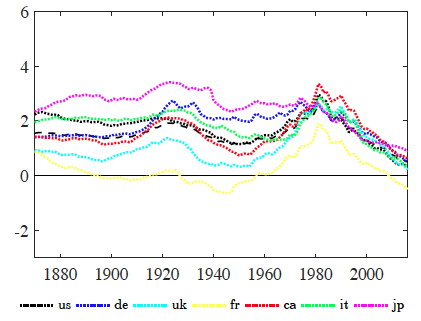
\includegraphics{Figures/delnegro12novfig4.png}
}

\end{center}
\caption{Substantial declines in `long run value' of \textit{real} rates in recent times, across many countries, Source: \href{https://voxeu.org/article/global-trends-interest-rates}{NY Fed}}
\end{figure}

\end{frame}

%-------------------------------------------------------

%-------------------------------------------------------

\begin{frame}{Real rates have declined to historically low levels}

The debate over falling real rates often refers to the long run `neutral' rate as $r^{\ast}$ or `r star'
\begin{itemize}
\item	From the reading list
	\begin{itemize}
	\item	Laubach and Williams (2015),
	\item	Williams (2018)
	\end{itemize}
\item	Also see \href{https://voxeu.org/article/global-trends-interest-rates}{here}, \href{https://voxeu.org/article/causes-and-consequences-persistently-low-interest-rates}{here} and \href{https://www.niesr.ac.uk/sites/default/files/publications/Box\%20A\%20-\%20Decline\%20interest\%20rates.pdf}{here}
\end{itemize}	

\vspace{2mm}
Connected to the broader debate on `secular stagnation'
\begin{itemize}
\item	Some argue US GDP trend growth $\downarrow$ from $3.5\%$ to $1.9\%$
\item	Collection of essays \href{https://voxeu.org/content/secular-stagnation-facts-causes-and-cures}{here} (if you're interested)
\end{itemize}

\end{frame}

%-------------------------------------------------------

%-------------------------------------------------------
	
\begin{frame}{Falling nominal rates}

Recall Fisher equation $i_{t} = r_{t} + E_{t}[\pi_{t+1}]$
\begin{itemize}
\item	If inflation expectations are stable (or falling), $i_{t}$ will fall with $r_{t}$
\end{itemize}

\vspace{2mm}
A shock (say, negative innovation to $Z_{t}$) may require $r_{t}$ to be lowered as part of optimal policy
\begin{itemize}
\item	$r^{\ast} \downarrow$ problematic if $\pi$ too low for $r_{t}<0$ given $i_{t}\geq0$
\item	Arises if desired $r_{t}$ (implied by a Taylor rule, perhaps) $< -E_{t}[\pi_{t+1}]$
\end{itemize}

\vspace{2mm}
Why is it typically thought $i_{t}\geq0$?
\begin{itemize}
\item	Option to hold cash, which earns a $0$ net nominal return
\item	Zero is better than negative!
%\item	Though we have seen moderately negative rates in some European countries recently - active debaet\ldots
\end{itemize}

\vspace{2mm}
During Great Recession and afterwards, standard policy rules $\Rightarrow$ negative nominal rates were necessary
\begin{itemize}
\item	U.S. and other countries hit the \emph{Zero Lower Bound}
\end{itemize}

\end{frame}

%-------------------------------------------------------

%-------------------------------------------------------
	
\begin{frame}{Nominal rates have declined to historically low levels}

\begin{figure}
\begin{center}

\resizebox{0.65\textwidth}{!}{%
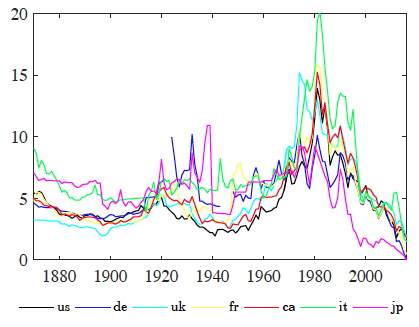
\includegraphics{Figures/delnegro12novfig1.png}
}

\end{center}
\caption{Substantial declines in rates in recent times, across many countries, Source: \href{https://voxeu.org/article/global-trends-interest-rates}{NY Fed} and \href{http://www.macrohistory.net/data}{Jorda \textit{et al's} Macrohistory Database}}
\end{figure}

\end{frame}

%-------------------------------------------------------

%-------------------------------------------------------
	
\begin{frame}{ZLB - short rates constrained}

\begin{figure}
\begin{center}

\resizebox{0.65\textwidth}{!}{%
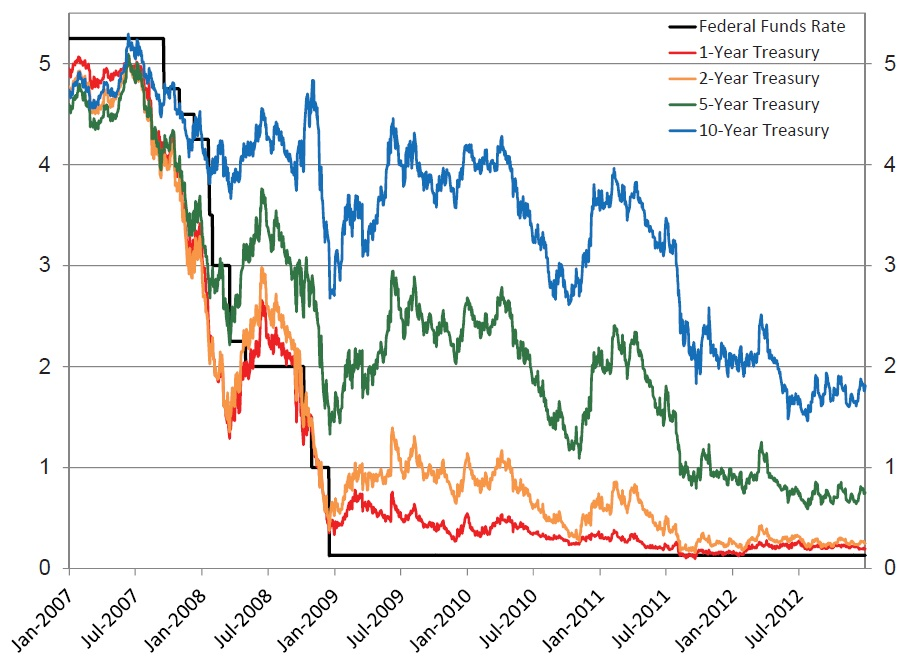
\includegraphics{Figures/williams_swanson_ZLB_frbsf_wp_long_term_rates.jpg}
}

\end{center}
\caption{Fed funds rate target and 1-, 2-, 5- and 10-year zero-coupon Treasury yields. Source: Federal Reserve Board and the Gurkaynak, Sack and Wright (2007) online dataset}
\end{figure}

\end{frame}

%-------------------------------------------------------

%-------------------------------------------------------
	
\begin{frame}{ZLB - inflation (and expectations?) declining}

\begin{figure}
\begin{center}

\resizebox{0.75\textwidth}{!}{%
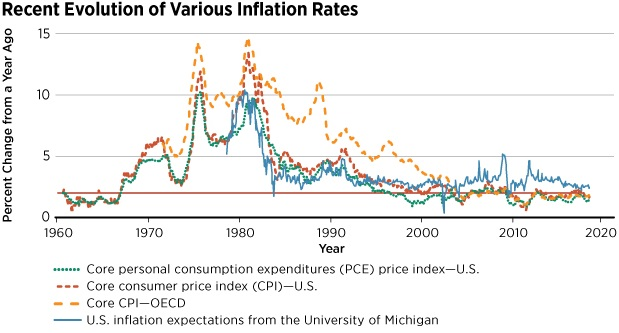
\includegraphics{Figures/Sanchez_fig1.jpg}
}

\end{center}
\caption{Declining U.S. inflation rate and expectations (red line is Fed's inflation target of $2\%$, Source: \href{https://www.stlouisfed.org/publications/regional-economist/first-quarter-2018/why-inflation-so-low}{St. Louis Fed}}
\end{figure}

\end{frame}

%-------------------------------------------------------

%-------------------------------------------------------
	
\begin{frame}{ZLB - short rates constrained}

To re-emphasize\ldots
\begin{itemize}
\item	Suppose $E_{t}[\pi_{t+1}]\leq \pi_{low}$
\item	Then real rate is constrained: $r_{t}\geq -\pi_{low}$ (as $i_{t}\geq 0$)
\item	Imagine $\pi_{low}=0$ then cannot set real rate negative (which has frequently helped stimulate the economy in other recessions)
\end{itemize}

\vspace{2mm}
Intuitively, monetary policy remains tight when it should be loose
\begin{itemize}
\item	CB cannot implement the responses in $r_{t}$ that we discussed earlier
\item	Theoretical possibility of being trapped in a deflationary spiral
\item	Scary - scan sections of \href{http://web.mit.edu/krugman/www/spiral.html}{Krugman reading} (up to and including `Adding the liquidity trap')
\end{itemize}

\vspace{2mm}
Useful readings for this topic
\begin{itemize}
\item	\href{https://www.brookings.edu/wp-content/uploads/2017/03/5_kileyroberts.pdf}{Kiley and Roberts (2017)} - Some of this too difficult but read the early sections - it contains nice overviews
\item	\href{https://www.brookings.edu/blog/ben-bernanke/2017/04/12/how-big-a-problem-is-the-zero-lower-bound-on-interest-rates/}{Bernanke (2017, `How big a problem\ldots)'}
\end{itemize}

\end{frame}

%-------------------------------------------------------

%-------------------------------------------------------
	
\begin{frame}{Is there anything we can do?}

\begin{itemize}
\item	Yes, maybe
	\begin{itemize}
	\item	Ask the Japanese how hard it is, and the current Fed and ECB policymakers how they feel about the situation right now\ldots
	\item	A lot of discussion of \textit{possible} new operating frameworks for Fed (e.g. price level targeting)
	\item	See \href{https://www.brookings.edu/research/monetary-policy-in-a-new-era/}{Bernanke (2017, `Mon. pol. in a new era')} and \href{https://www.brookings.edu/blog/up-front/2018/09/14/comments-on-monetary-policy-at-the-effective-lower-bound/}{Yellen (2018)}
	\end{itemize}
\vspace{2mm}
\item	Various possibilities - a few are\ldots
	\begin{itemize}
	\item	Forward guidance
	\item	QE
	\item	Fiscal expansion
	\item	Raise inflation target
	\item	Introduce price-level targeting
	\end{itemize}
\end{itemize}

\end{frame}

%-------------------------------------------------------

%-------------------------------------------------------
	
\begin{frame}{Forward guidance}

Setting ZLB aside, recall our DIS equation from the NK lecture
\begin{eqnarray*}
\tilde{y}_{t} &=& E_{t} \left[ \tilde{y}_{t+1} \right] - \frac{1}{\sigma} \left(i_{t} - E_{t}\left[ \pi_{t+1} \right]  - r^{n}_{t} \right) \label{eqn:dyn_IS} \\
&=& -\frac{1}{\sigma} \sum\limits_{k=0}^{\infty} E_{t}[ r_{t+k}  - r^{n}_{t+k} ] \nonumber \\
&=& -\frac{1}{\sigma} \sum\limits_{k=0}^{\infty} E_{t}[ i_{t+k} -  (r^{n}_{t+k} + \pi_{t+k+1}) ] \nonumber
\end{eqnarray*}
where we used the Fisher equation and $E_{t}[E_{t+k}[\pi_{t+k+1}]]= E_{t}[\pi_{t+k+1}]$

\vspace{2mm}
Current output gap reflects current and expected values of $i_{t}$, $\pi_{t}$ $r^{n}_{t}$
\begin{itemize}
\item	Assume, as \textit{in our simple NK model}, $y^{n}_{t}$ is independent of $v_{t}$ and $z_{t}$
\item	If the C.B. sets \textit{or is expected} to set $i_{t}$ in a particular way then it may influence the output gap - also may be able to influence $E_{t}[\pi_{t+k}]$
\end{itemize}

\end{frame}

%-------------------------------------------------------

%-------------------------------------------------------
	
\begin{frame}{Williams and Swanson 2013 - Long rate sensitivity to news}

\begin{figure}
\begin{center}

\resizebox{0.35\textwidth}{!}{%
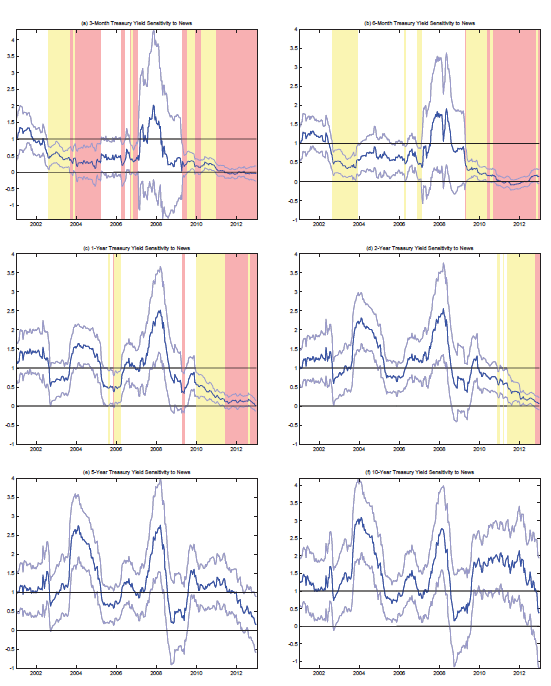
\includegraphics{Figures/williams_swanson_sensitive_guide_frbsf_wp_long_term_rates.png}
}

\end{center}
\caption{Sensitivity of Treasury yields to news (3-Mo, 6-Mo, 1-Y, 2-Y, 5-Y, 10-Y), Red and yellow indicate periods of insensitivitiy. Source: \href{https://pubs.aeaweb.org/doi/pdfplus/10.1257/aer.104.10.3154}{Swanson and Williams (2014)}}
\end{figure}

\end{frame}

%-------------------------------------------------------

%-------------------------------------------------------
	
\begin{frame}{Forward guidance}

\begin{equation*}
\tilde{y}_{t} = -\frac{1}{\sigma} \sum\limits_{k=0}^{\infty} E_{t}[ i_{t+k} -  (r^{n}_{t+k} + \pi_{t+k+1}) ]
\end{equation*}
\begin{itemize}
\item	Guidance about how rates will behave after period of ZLB can be influential if it is \textbf{credible}
\item	If CB can affect expectations of $i_{t+j}$ and $\pi_{t+j}$ \emph{in the future} then can influence economy even if currently at ZLB
	\begin{itemize}
	\item	See \textit{introductions} of papers on reading list and \href{https://www.frbsf.org/economic-research/files/SecretsShort-NBER-ch6-2008.pdf}{this classic}
	\item	Also see \href{https://uk.reuters.com/article/us-usa-fed-williams/feds-williams-makes-case-for-lower-for-longer-rates-idUKKCN1S91OE}{here}, \href{https://www.newyorkfed.org/newsevents/speeches/2019/wil190718}{here} and \href{https://www.brookings.edu/blog/up-front/2018/09/14/comments-on-monetary-policy-at-the-effective-lower-bound/}{here}
	\end{itemize}
\item	Some channels:
	\begin{itemize}
	\item	Many borrowing rates (e.g. mortgages) are at longer maturities and perhaps can be influenced
	\item	Might enhance confidence
	\item	Could induce depreciation in exchange rate - stimulating exports (and maybe raising inflation)
	\end{itemize}
\item	But\ldots theory is subtle/debatable
\end{itemize}

\end{frame}

%-------------------------------------------------------

%-------------------------------------------------------
	
\begin{frame}{Fed date-based guidance - powerful effect in 2011}

\begin{figure}
\begin{center}

\resizebox{0.35\textwidth}{!}{%
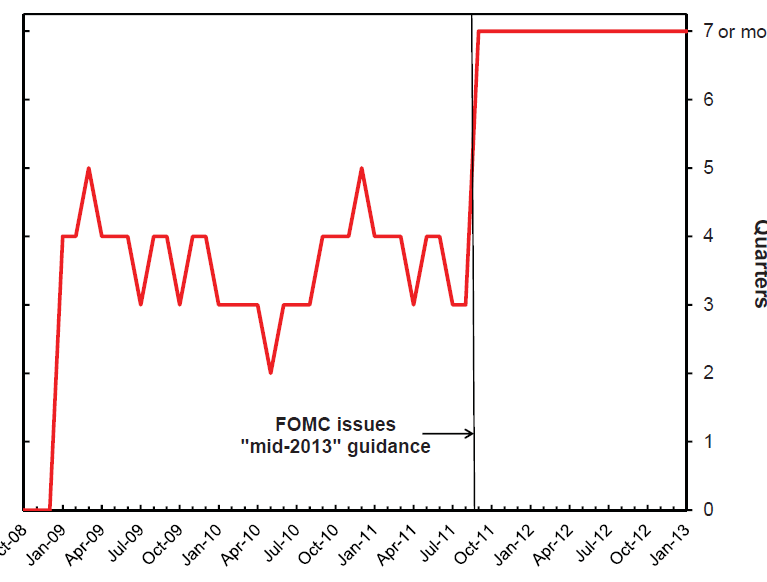
\includegraphics{Figures/williams_swanson_2013_guide_frbsf_wp_long_term_rates.png}
}

\end{center}
\caption{Effect of explicit date-based forward guidance (implemented in mid 201) on expected number of quarters until `lift-off' from ZLB, Source: Blue Chip and \href{https://pubs.aeaweb.org/doi/pdfplus/10.1257/aer.104.10.3154}{Swanson and Williams (2014)}}
\end{figure}

\begin{itemize}
\item	In 2011, economic conditions, \emph{`likely to warrant exceptionally low levels for the federal funds rate at least through mid-2013'}
\item	Compare with, less explicit, `indications that rates were likely to stay low \emph{`for some time'}
\end{itemize}

\end{frame}

%-------------------------------------------------------

%-------------------------------------------------------
	
\begin{frame}{Raising (or stabilizing?) inflation expectations}

Some people have suggested revisiting the Fed's interpretation of the `price stability' aspect of its \href{https://www.chicagofed.org/research/dual-mandate/dual-mandate}{`dual mandate'}
\begin{itemize}
\item	Fed pursues a $2\%$ inflation target, which was asserted before people fully grasped the scale of $r^{\ast}\downarrow$
\item	Some people think the decline has been from $3.5\%$ to approx $0,5\%$
\item	Thus, in `steady state' the nominal rate probably now sits around $2.5\%-3.0\%$, rather than $5.5\%$ as previously
\item	Means that there is less room to cut in a recession (before hitting ZLB)
\end{itemize}

\vspace{2mm}
See \href{https://www.jstor.org/stable/2138238}{Bernanke and Mishkin (1997)} on reading list or \href{https://www.imf.org/external/pubs/ft/fandd/basics/target.htm}{here} for more on inflation targeting
\begin{itemize}
\item	Recall also our conventional monetary policy price stability discussion
\item	Due to quality improvements etc. $2.0\%$ rather than literally $0\%$ is interpreted as price stability
\end{itemize}

\end{frame}

%-------------------------------------------------------

%-------------------------------------------------------
	
\begin{frame}{Raising (or stabilizing?) inflation expectations}

One option discussed is to raise the inflation target (see chapter 1 \href{https://www.niesr.ac.uk/sites/default/files/publications/Renewing\%20our\%20Monetary\%20Vows\%20text.pdf}{here})
\begin{itemize}
\item	What seems increasingly to be proposed instead is `price level targeting'
\item	See \href{https://www.jstor.org/stable/2601112}{Svensson (1999)}, \href{https://www.brookings.edu/research/monetary-policy-in-a-new-era/}{Bernanke (2017)} (easier) and \href{https://www.investopedia.com/terms/p/price_level_targeting.asp}{Investopedia} (easiest)
\end{itemize}

\vspace{2mm}
Main difference between price level and inflation targeting is that price level targeting implies a promise to adjust for past inflation misses
\begin{itemize}
\item	Under inflation targeting: If you suffer a few periods of sub-target inflation, that doesn't change the aim to hit target inflation from today onwards
\item	Under price-level targeting: If you suffer a few periods of sub-target inflation, you aim for higher than target inflation until you're back on the initial price path
\end{itemize}

\end{frame}

%-------------------------------------------------------

%-------------------------------------------------------
	
\begin{frame}{Raising (or stabilizing?) inflation expectations}

\begin{figure}
\begin{center}

\resizebox{0.50\textwidth}{!}{%
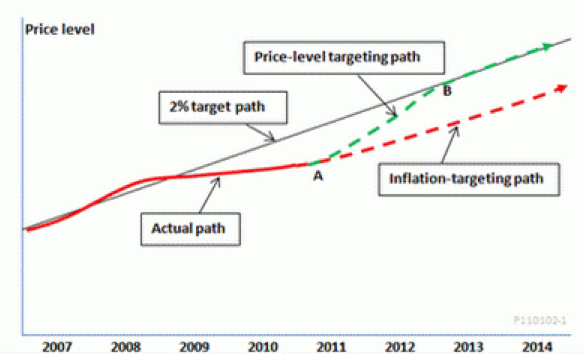
\includegraphics{Figures/price-level-target11.png}
}

\end{center}
\caption{Price and inflation behavior under inflation targeting and price level targeting, Source: \href{https://econfix.wordpress.com/2011/07/02/price-level-targeting-and-inflation-targeting-part-1-the-theory/}{Econfix}}
\end{figure}

\begin{itemize}
\item	So? Because of ZLB we are particularly concerned with the level of inflation and even downward drift in inflation expectations
\item	PLT `could' be a credible way of promising higher inflation in the near term, helping to lower real rates now, thus stimulating the economy
\end{itemize}

\end{frame}

%-------------------------------------------------------

%-------------------------------------------------------
	
\begin{frame}{Quantitative Easing}

\begin{figure}
\begin{center}

\resizebox{0.55\textwidth}{!}{%
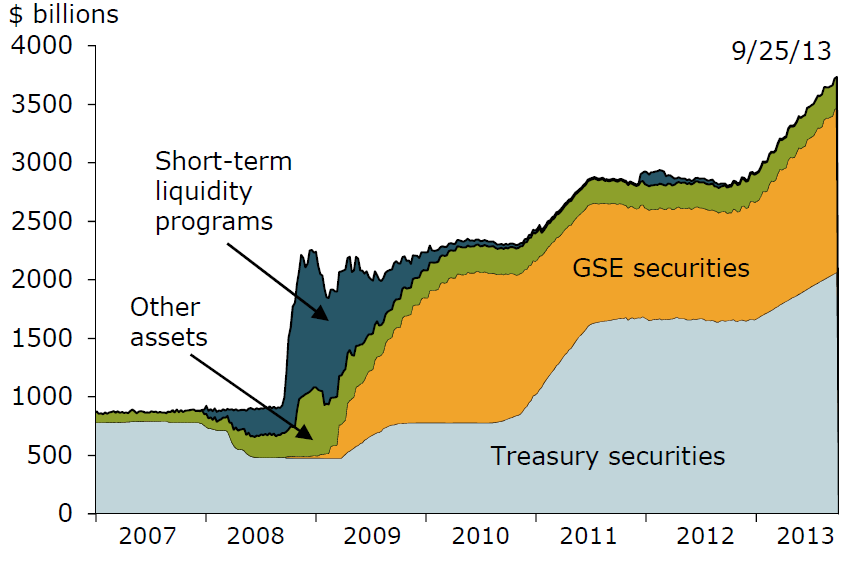
\includegraphics{Figures/williams_el_fed_balance_sheet.png}
}

\end{center}
\caption{Federal Reserve asset holdings, Source: Federal Reserve Board.}
\end{figure}

Fed massively expanded its balance sheets to purchase assets
\begin{itemize}
\item	Initially some liquidity programs - but most importantly QE
\item	Nice readable review \href{https://www.frbsf.org/economic-research/publications/economic-letter/2018/december/review-of-unconventional-monetary-policy/}{here} with good bibliography if you're interested
\end{itemize}

\end{frame}

%-------------------------------------------------------

%-------------------------------------------------------
	
\begin{frame}{Quantitative Easing}

QE1 (December 2008)
	\begin{itemize}
	\item	$\$600bn$ of \href{https://www.investopedia.com/terms/a/agency-mbs-purchase.asp}{agency MBS} and debt - initially sterilized
	\item	Later $\$750bn$ more + $\$300bn$ Treasuries - not sterilized (QE up and running)
	\end{itemize}
\vspace{3mm}
QE2 (November 2010)
	\begin{itemize}
	\item	$\$600bn$ of long-dated Treasuries ($BS\uparrow$)
	\end{itemize}

\end{frame}

%-------------------------------------------------------

%-------------------------------------------------------
	
\begin{frame}{Quantitative Easing}

Operation Twist (2011)
	\begin{itemize}
	\item	Purchase $\$400bn$ bonds with maturities $6$ to $30$ years, using proceeds from selling bonds with maturities less than $3$ years
	\item	Limited impact on size of balance sheet - changing composition
	\item	Lengthened average maturity and `removed duration' from market
	\item	Later extended with further $\$267bn$
	\item	Eventually ran out of short dated to sell
	\end{itemize}
\vspace{2mm}
QE3 (2012)
	\begin{itemize}
	\item	Open ended commitment to purchase $\$40bn$ agency MBS until labor market improved
	\item	Later added up $\$45bn$ long dated Treasury purchases per month
	\end{itemize}

\end{frame}

%-------------------------------------------------------

%-------------------------------------------------------
	
\begin{frame}{Balance sheet decomposition - asset class}

\begin{figure}
\begin{center}

\resizebox{0.80\textwidth}{!}{%
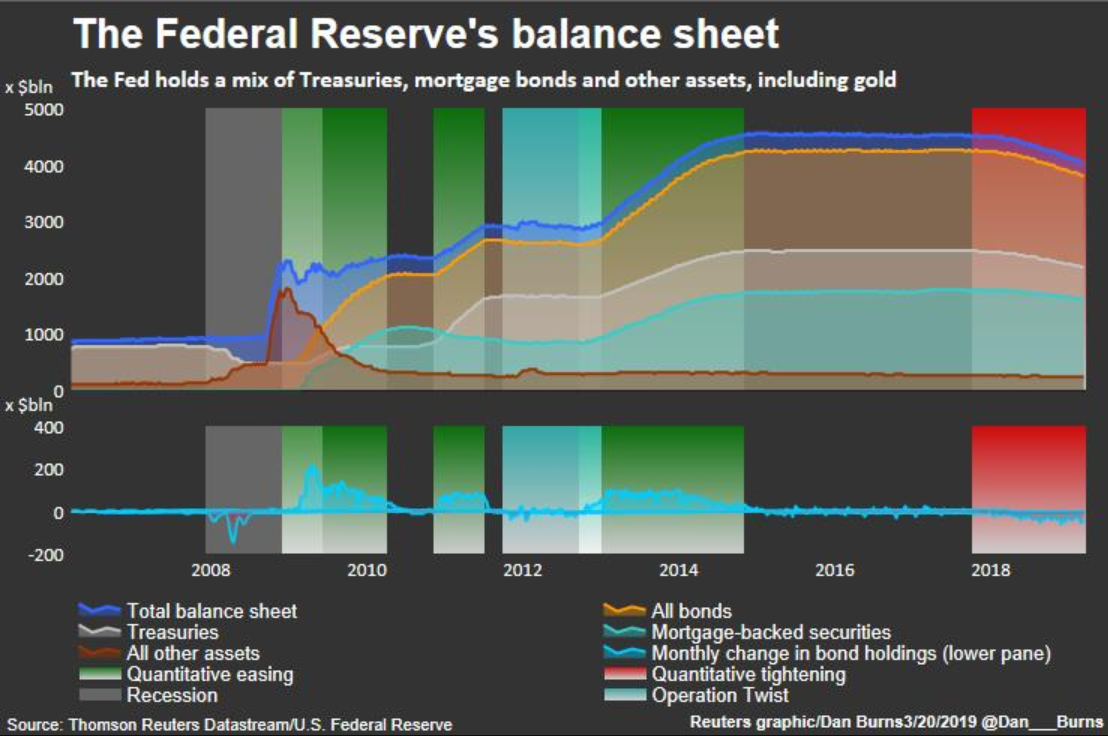
\includegraphics{Figures/fed_bs_decomp.png}
}

\end{center}
\end{figure}

\end{frame}

%-------------------------------------------------------

%-------------------------------------------------------
	
\begin{frame}{Balance sheet decomposition - maturity}

\begin{figure}
\begin{center}

\resizebox{0.80\textwidth}{!}{%
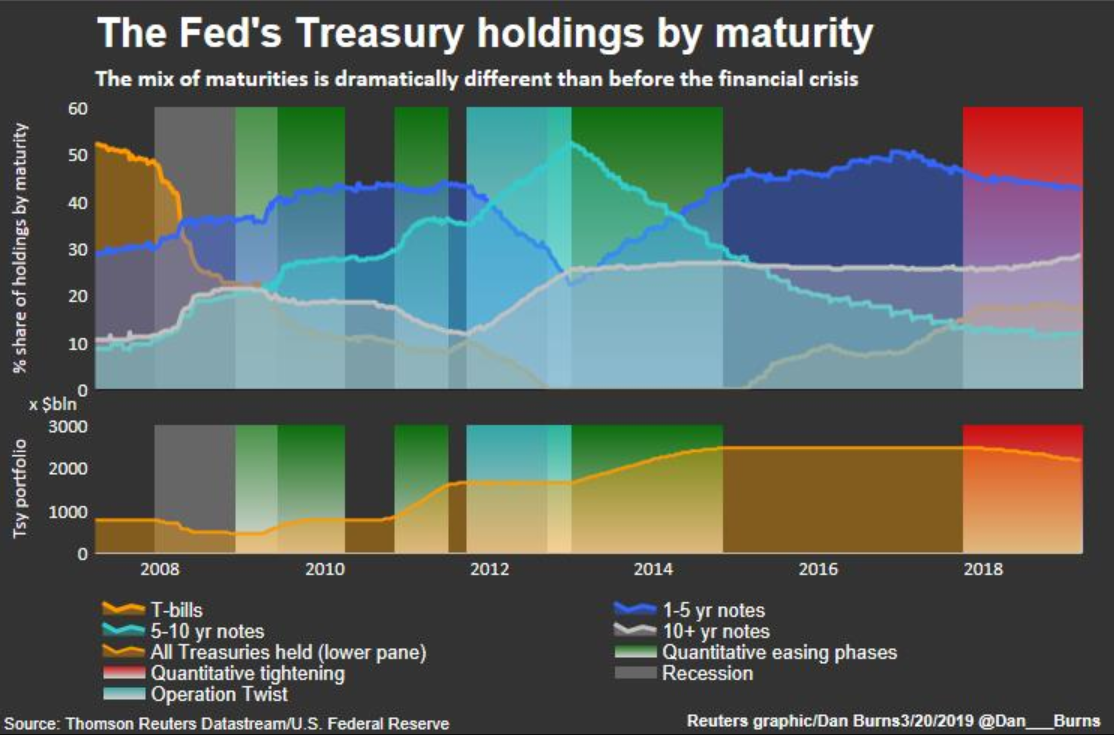
\includegraphics{Figures/fed_bs_decomp_maturity.png}
}

\end{center}
\end{figure}

\end{frame}

%-------------------------------------------------------

%-------------------------------------------------------
	
\begin{frame}{Channels}

Main intended channels
	\begin{itemize}
	\item	Drive down long rates (similar aim to FG) - paper \href{https://academic.oup.com/ej/article/122/564/F385/5079473}{here} if interested
	\item	Induce substitution into other - riskier - assets (e.g. mortgages, C\&I)
	\item	Stimulate stock market (aiding wealth and confidence)
	\item	See Gagnon papers,, D'Amico and Carpenter, plus \href{https://www.piie.com/system/files/documents/pb18-19.pdf}{this nice overview}
	\end{itemize}
\vspace{2mm}
Theoretical basis somewhat unclear (still)
	\begin{itemize}
	\item	But empirically, rates did seem to drop - at least around impact
	\item	VAR analysis and other approaches also suggest effect on economy
	\end{itemize}
\vspace{2mm}
Possible additional channels
	\begin{itemize}
	\item	Conveying commitment or signaling future $i_{t}^{e}$ policy - see \href{https://www.ijcb.org/journal/ijcb14q3a7.htm}{here}
	\item	Weakening exchange rate (though not primary aim)
	\item	Solidifying bank balance sheets (from rising asset prices)
	\end{itemize}

\end{frame}

%-------------------------------------------------------

%-------------------------------------------------------
	
\begin{frame}{Stimulating risk assets? Dow Jones}

\begin{figure}
\begin{center}

\resizebox{0.80\textwidth}{!}{%
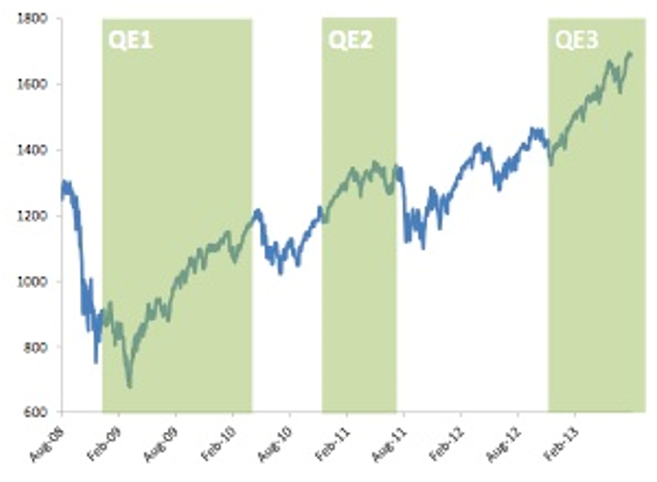
\includegraphics{Figures/Dow_Jones_QE123.png}
}

\end{center}
\end{figure}

\end{frame}

%-------------------------------------------------------

%-------------------------------------------------------
	
\begin{frame}{Fiscal policy?}

Big increase in `G' can `shift' the IS curve far to the `right'
\begin{itemize}
\item	Effectively a large demand shock that raises the $r_{t}$ that should be sought by the CB
\item	Blasts the economy out of the ZLB
\end{itemize}

\vspace{2mm}
Is it that easy?
	\begin{itemize}
	\item	Not necessarily
	\item	Ricardian equivalence and expectations of future taxes (if spending is deficit financed)
	\item	May mean a loss of confidence or leave expected effect on permanent income $\approx$ zero
	\item	Countries already in a bad fiscal position (esp. if they've bailed out banks) may not be `allowed' by the markets to borrow to fund spending - and raising taxes is difficult in recession
	\end{itemize}
	
\end{frame}

%----------------------------------------------------------------------------
%Main body
\appendix
%-------------------------------------------------------

%-------------------------------------------------------

\begin{frame}

\begin{center}
{\LARGE Escape Slides}
\end{center}

\end{frame}

%-------------------------------------------------------

%-------------------------------------------------------
	
\begin{frame}[label=efficiency_escape]{An efficient benchmark}

Loosely speaking, efficiency $\Rightarrow$ MRS = MRT which in this case implies
\[
-\frac{U_{n,t}}{U_{c,t}} = MPN_{t}
\]

But we know in the flex price equilibrium
\[
-\frac{U_{n,t}}{U_{c,t}} \stackrel{\textcolor{red}{HHOLD}}= \frac{W_{t}}{P_{t}}\stackrel{\textcolor{red}{FIRM}}= \frac{MPN_{t}}{\mathcal{M}} < MPN_{t}
\]

\end{frame}

%-------------------------------------------------------

%-------------------------------------------------------
	
\begin{frame}{An efficient benchmark}

Employment subsidy at rate $\tau$ $\Rightarrow$ effective wage paid by firms is $(1-\tau)W_{t}$

\vspace{2mm}
\begin{itemize}
\item	Then firm optimality implies
\[
\frac{W_{t}(1-\tau)}{P_{t}}= \frac{MPN_{t}}{\mathcal{M}}
\]
\item	So that, if $\tau$ is set to be $=\varepsilon^{-1}$ we recover
\[
\frac{W_{t}}{P_{t}}= MPN_{t}
\]
\end{itemize}

Refer back to problem set 2 where essentially the same issue was discussed thoroughly

\hyperlink{efficiency}{\beamergotobutton{Back}}

\end{frame}

\end{document}
